\documentclass{article}

\usepackage{graphicx}
\usepackage{subfig}
\usepackage{multirow}
\usepackage{subcaption}


\title{{\bf Supplementary Material:} \\A causal web between chronotype and metabolic health traits}
https://www.overleaf.com/project/605b6416422edc98436c7254
\author{}
\date{}

\begin{document}
\maketitle

Appendix 1: AppendixTable1EpigraphDBIVWresults.xlsx. EpiGraphDB data downloaded to produce Figure 2.

Appendix 2: AppendixTable2StudyCharacteristics.xlsx.
SNP-level information on all 10 studies analyzed needed to reproduce analyses of these 10 studies. to supplementary scatter plots, leave-one-out plots, and Figures 3-5 and supplementary figures.

Appendix 3: AppendixTable3MRAnalysisResults.xlsx. Summary level results for each of the 10 MR analyses, including leave-one-out statistics, MR-Egger statistics, and all MR statistics. Used to produce supplementary scatter plots, leave-one-out plots, and Figures 3-5 and supplementary figures. 

Appendix 4: AppendixTable4ConfounderGraph.xlsx.
Statistics downloaded from EpiGraphDB needed to reproduce figures 6 and 7.




% omega 3 and total triglycerides
\begin{figure}[htbp]
     \centering
     \begin{subfigure}[b]{0.4\textwidth}
         \centering
         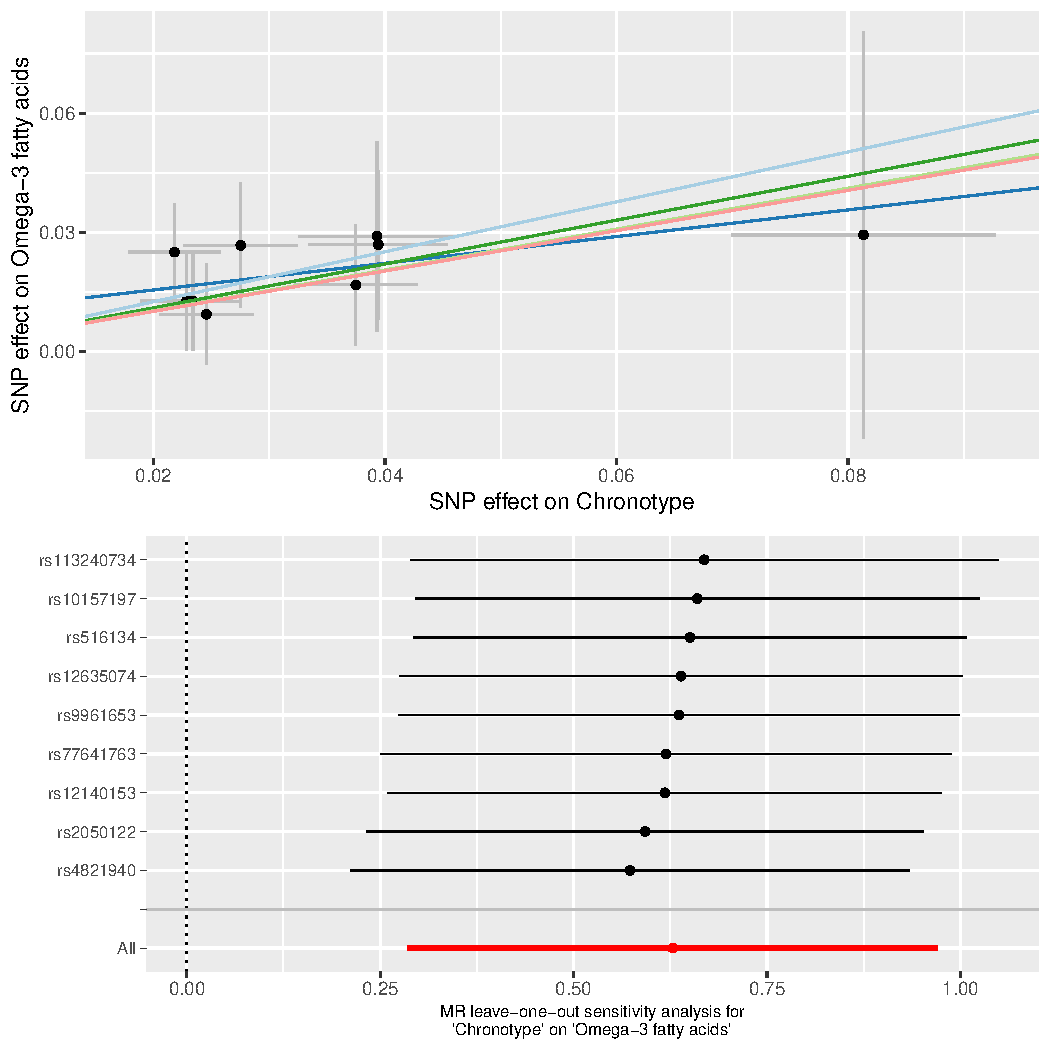
\includegraphics[width=0.4\textwidth]{Figs/Analysis2/Chronotype_vs_Omega-3_fatty_acids.Plots.pdf}
         %\caption{}
         \label{omega3}
     \end{subfigure}
     \begin{subfigure}[b]{0.4\textwidth}
         \centering
         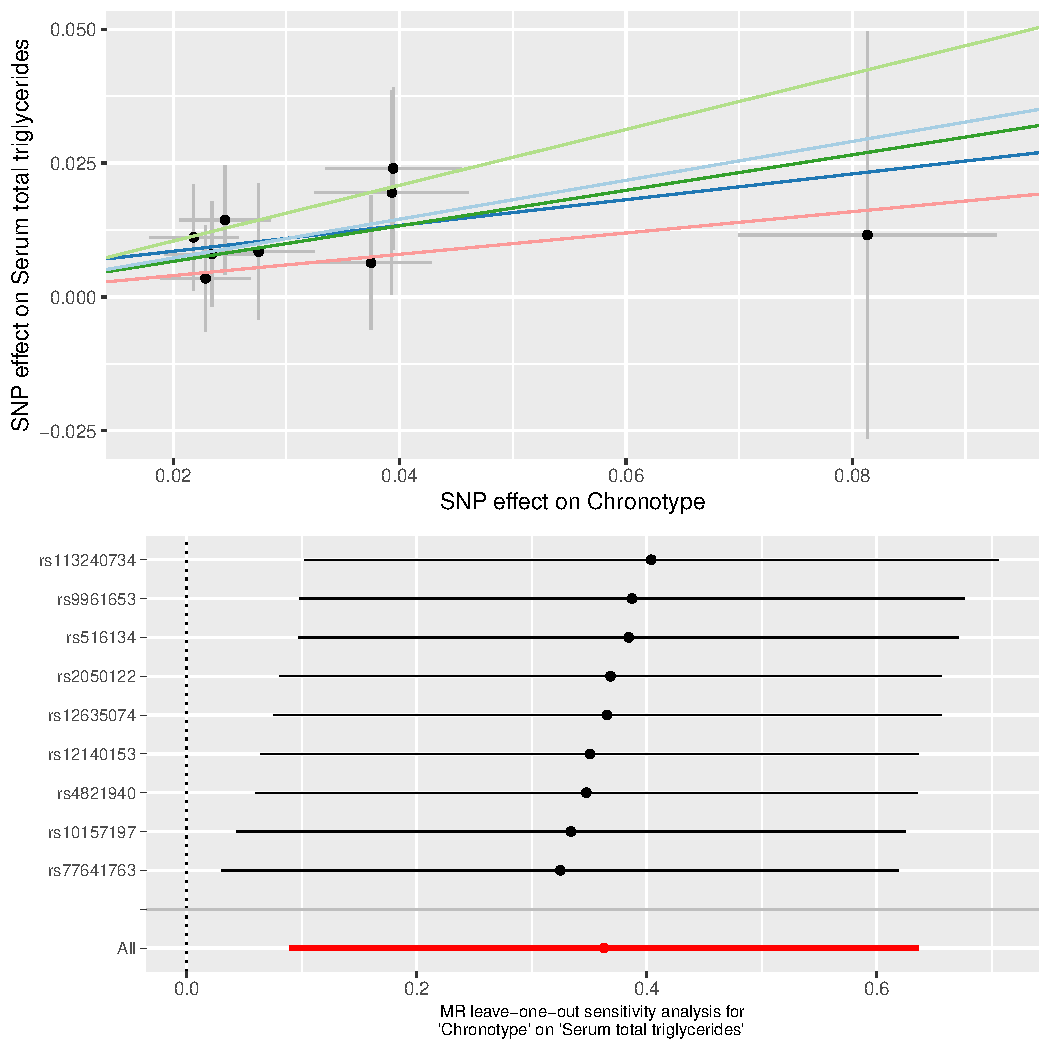
\includegraphics[width=0.4\textwidth]{Figs/Analysis2/Chronotype_vs_Serum_total_triglycerides.Plots.pdf}
         %\caption{}
         \label{totalTG}
     \end{subfigure}
        \caption{Propensity to an evening chronotype causes increased omega-3 fatty acids (A) and serum total triglycerides (B). IVW, Weighted median, mode, weighted mode, and Egger regressions shown. Lower panels depict leave-one-out sensitivity analyses with the IVW method.}
        \label{omega3tgs}
\end{figure}

% total ffa and nicorandil
\begin{figure}[htbp]
     \centering
     \begin{subfigure}[b]{0.4\textwidth}
         \centering
         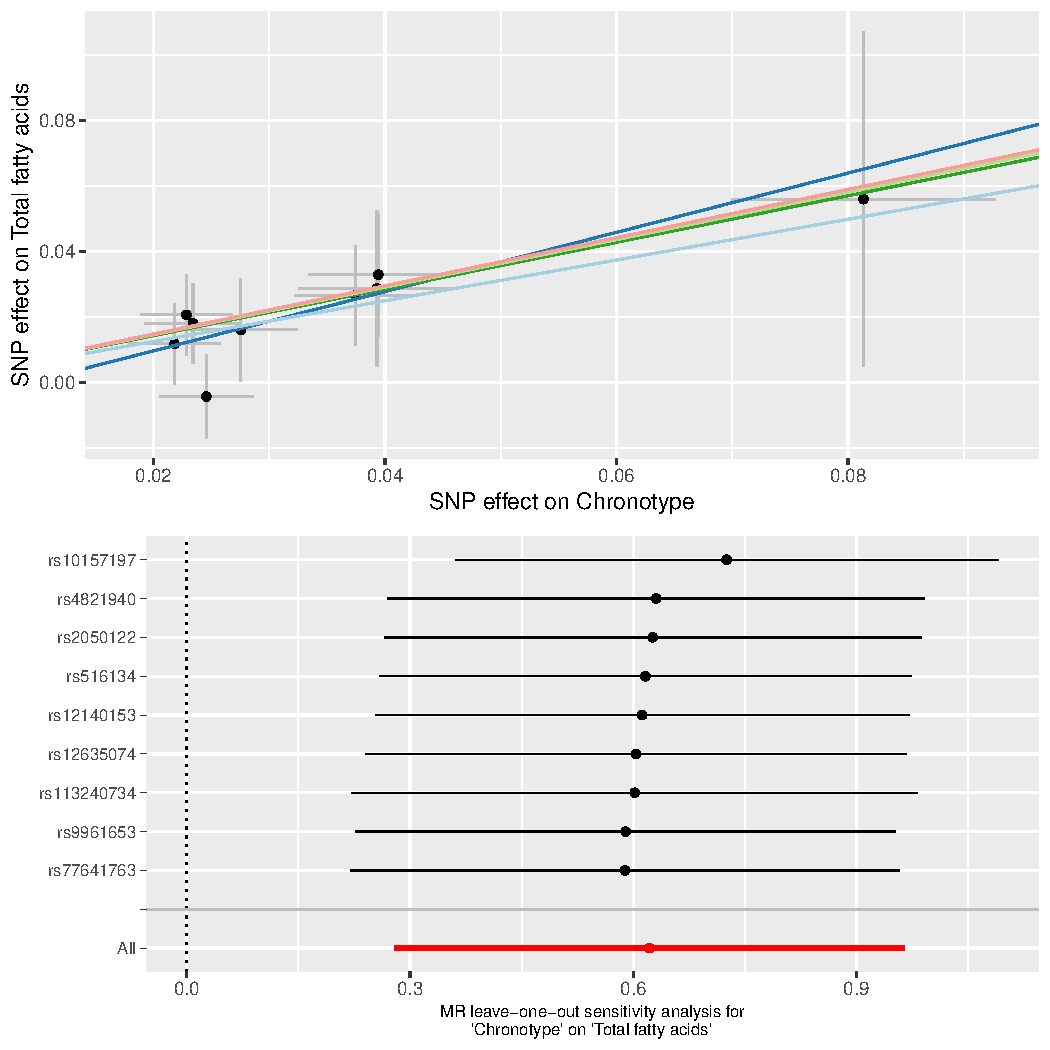
\includegraphics[width=\textwidth]{Figs/Analysis2/Chronotype_vs_Total_fatty_acids.Plots.pdf}
         \caption{}
         \label{tffa}
     \end{subfigure}
     \begin{subfigure}[b]{0.4\textwidth}
         \centering
         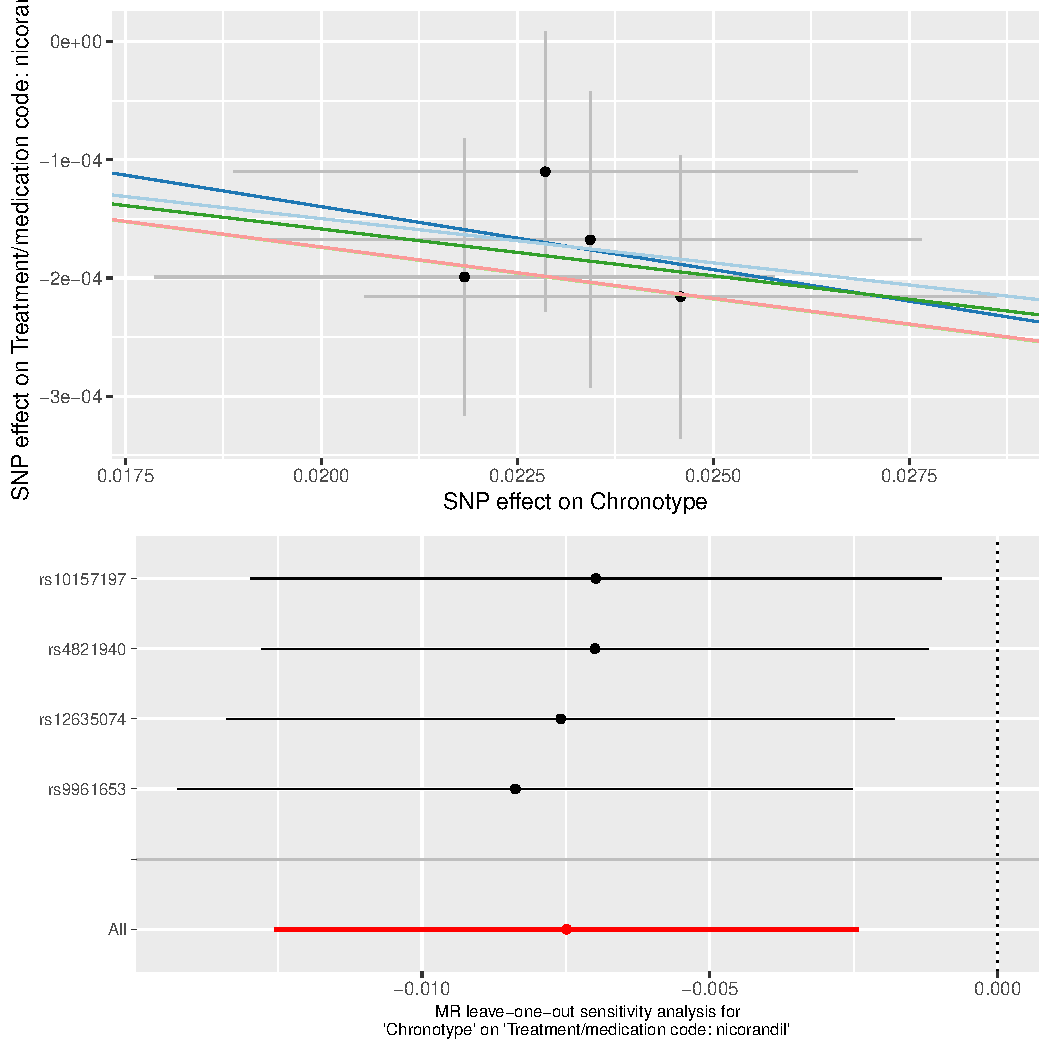
\includegraphics[width=\textwidth]{Figs/Analysis2/Chronotype_vs_Treatment_medication_code:_nicorandil.Plots.pdf}
         \caption{}
         \label{nicorandil}
     \end{subfigure}
        \caption{Chronotype causes increased total fatty acids (A) and and a decreased likelihood of treatment with nicorandil. IVW, Weighted median, mode, weighted mode, and Egger regressions shown. Lower panels depict leave-one-out sensitivity analyses with the IVW method.}
        \label{nicorandil}
\end{figure}


% total T2dm and alcohol
\begin{figure}[htbp]
     \centering
     \begin{subfigure}[b]{0.4\textwidth}
         \centering
         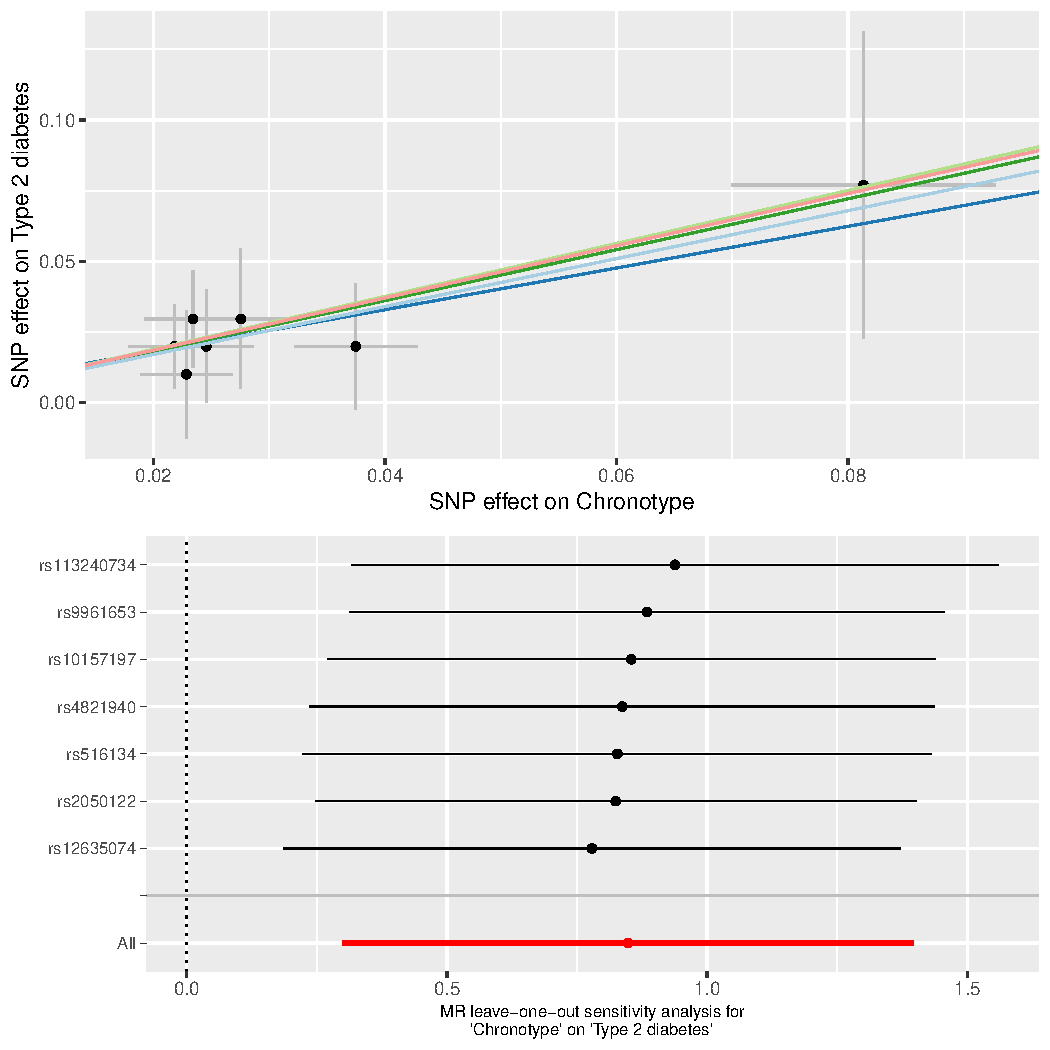
\includegraphics[width=\textwidth]{Figs/Analysis2/Chronotype_vs_Type_2_diabetes.Plots.pdf}
         \caption{}
         \label{t2dm}
     \end{subfigure}
     \begin{subfigure}[b]{0.4\textwidth}
         \centering
         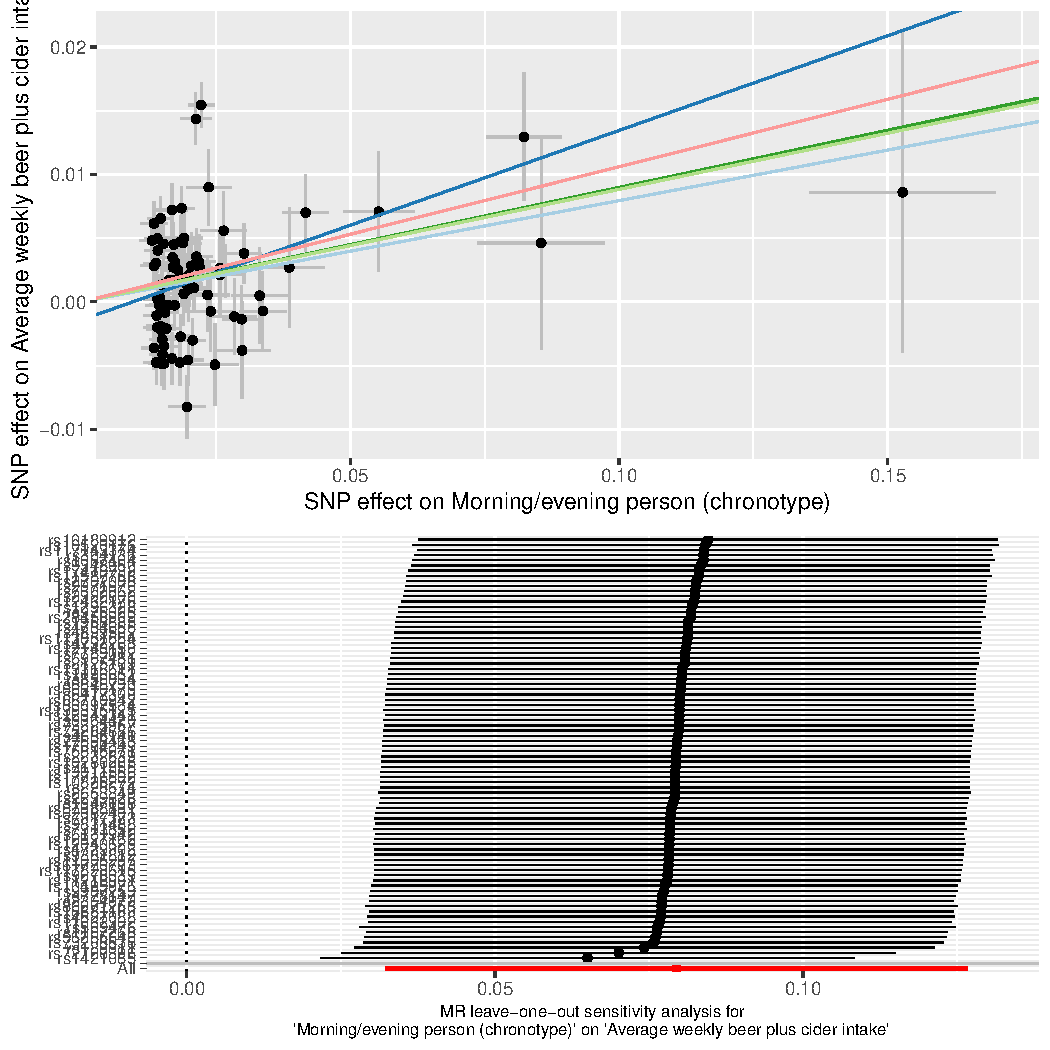
\includegraphics[width=\textwidth]{Figs/Analysis2/Morning_evening_person_(chronotype)_vs_Average_weekly_beer_plus_cider_intake.Plots.pdf}
         \caption{}
         \label{beer}
     \end{subfigure}
        \caption{Chronotype causes increased odds of a type 2 diabetes mellitus diagnosis (A) and and an increased weekly beer/cider intake. IVW, Weighted median, mode, weighted mode, and Egger regressions shown. Lower panels depict leave-one-out sensitivity analyses with the IVW method.}
        \label{t2dmalcohol}
\end{figure}

% total bp and tired
\begin{figure}[htbp]
     \centering
     \begin{subfigure}[b]{0.4\textwidth}
         \centering
         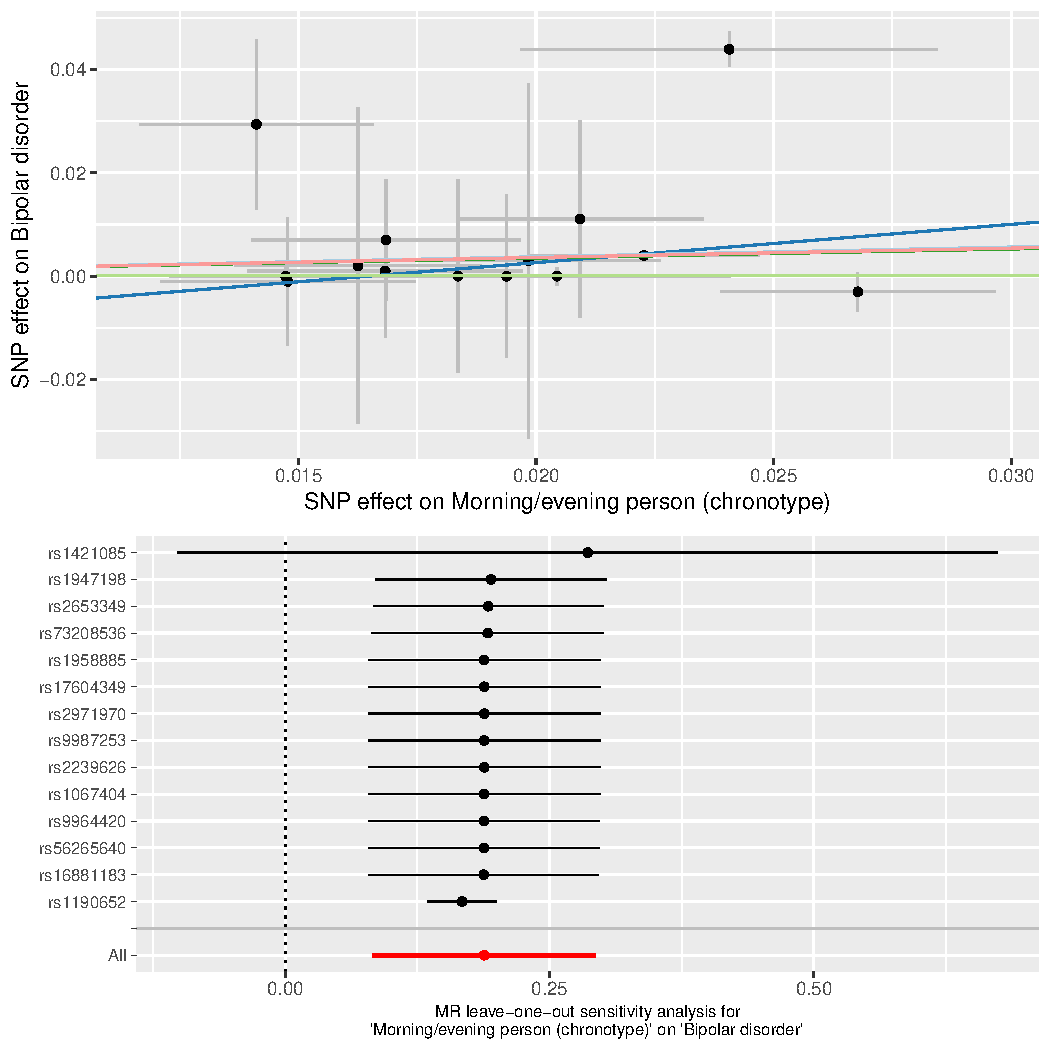
\includegraphics[width=\textwidth]{Figs/Analysis2/Morning_evening_person_(chronotype)_vs_Bipolar_disorder.Plots.pdf}
         \caption{}
         \label{t2dm}
     \end{subfigure}
     \begin{subfigure}[b]{0.4\textwidth}
         \centering
         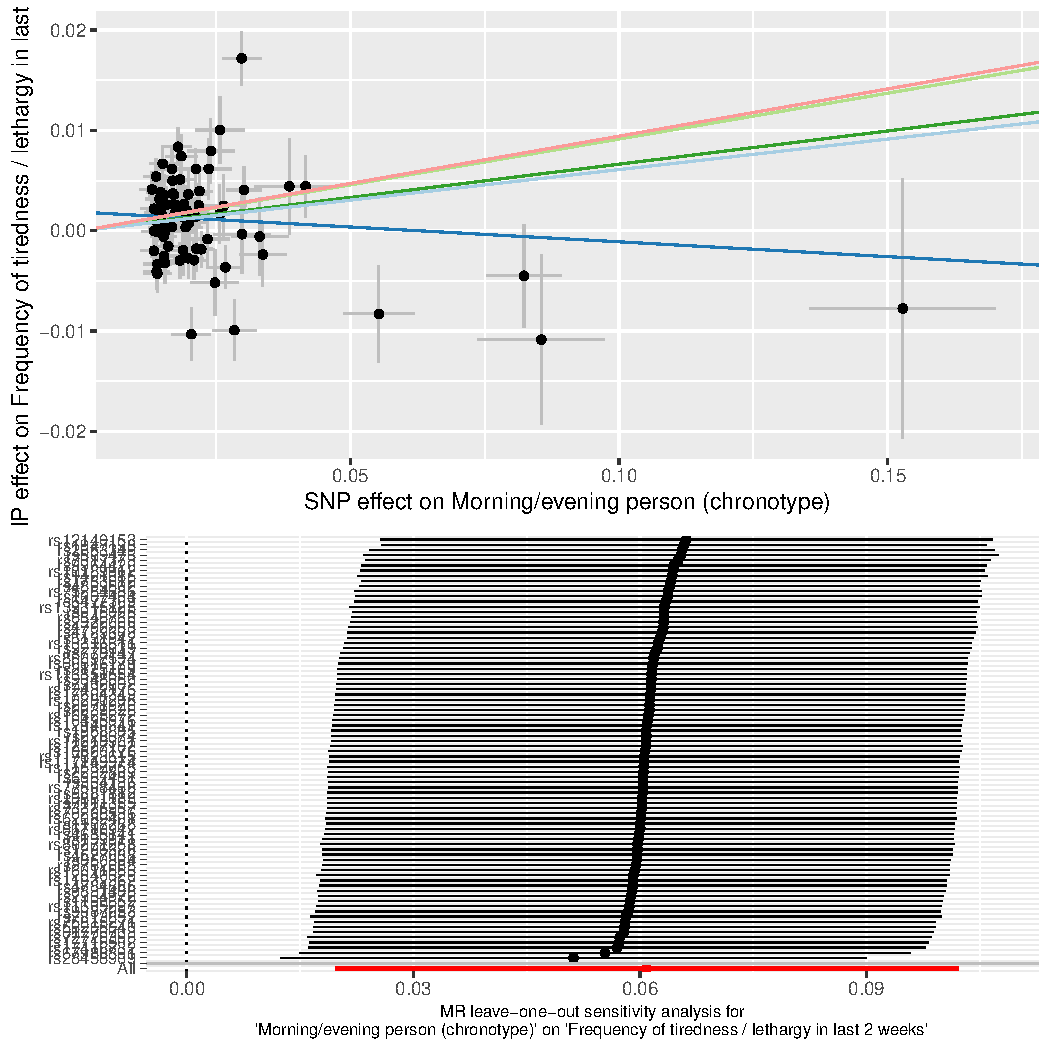
\includegraphics[width=\textwidth]{Figs/Analysis2/Morning_evening_person_(chronotype)_vs_Frequency_of_tiredness___lethargy_in_last_2_weeks.Plots.pdf}
         \caption{}
         \label{beer}
     \end{subfigure}
        \caption{An evening chronotype contributes to a bipolar disorder diagnosis (A) and self-reported lethargy. IVW, Weighted median, mode, weighted mode, and Egger regressions shown. Lower panels depict leave-one-out sensitivity analyses with the IVW method.}
        \label{bplethargy}
\end{figure}

% total test and wakingearly
\begin{figure}[htbp]
     \centering
     \begin{subfigure}[b]{0.4\textwidth}
         \centering
         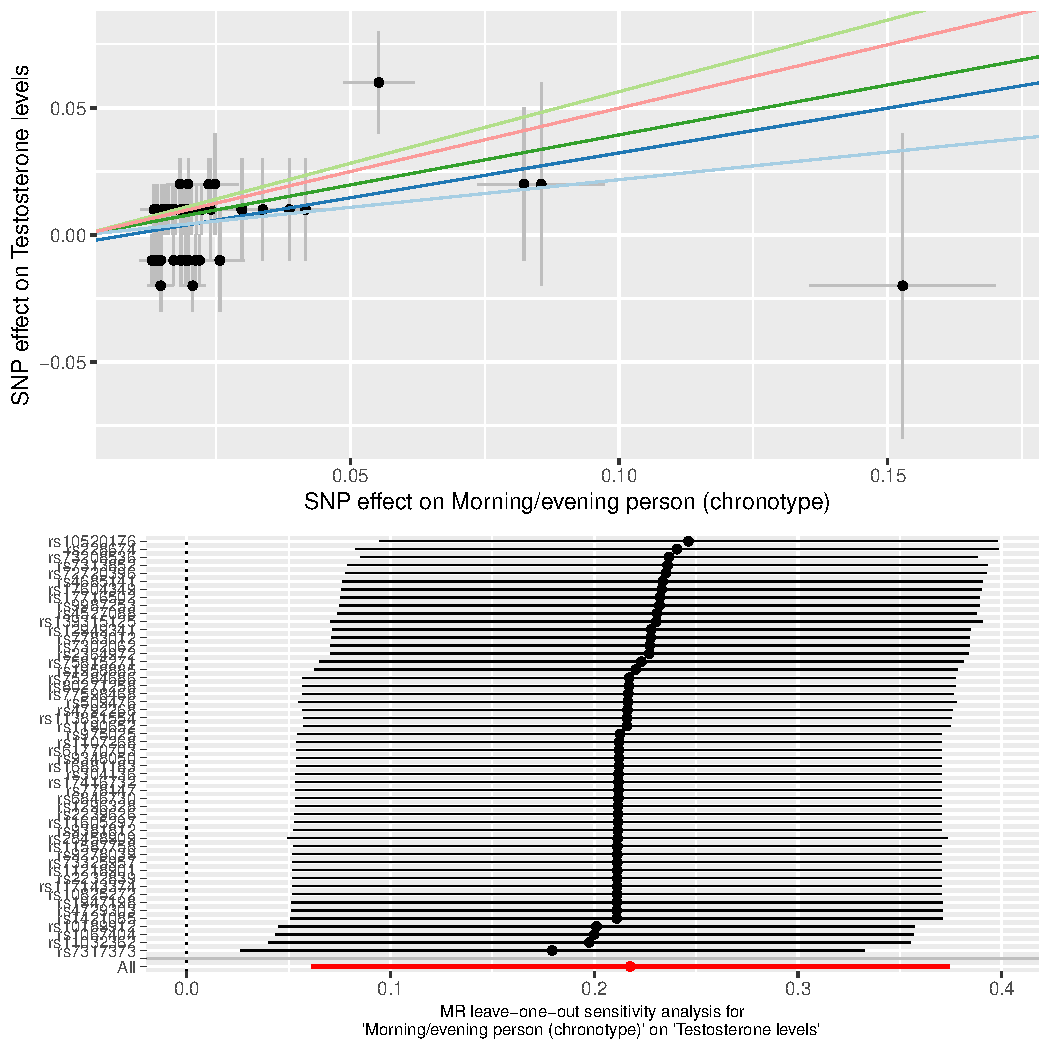
\includegraphics[width=\textwidth]{Figs/Analysis2/Morning_evening_person_(chronotype)_vs_Testosterone_levels.Plots.pdf}
         \caption{}
         \label{testosterone}
     \end{subfigure}
     \begin{subfigure}[b]{0.4\textwidth}
         \centering
         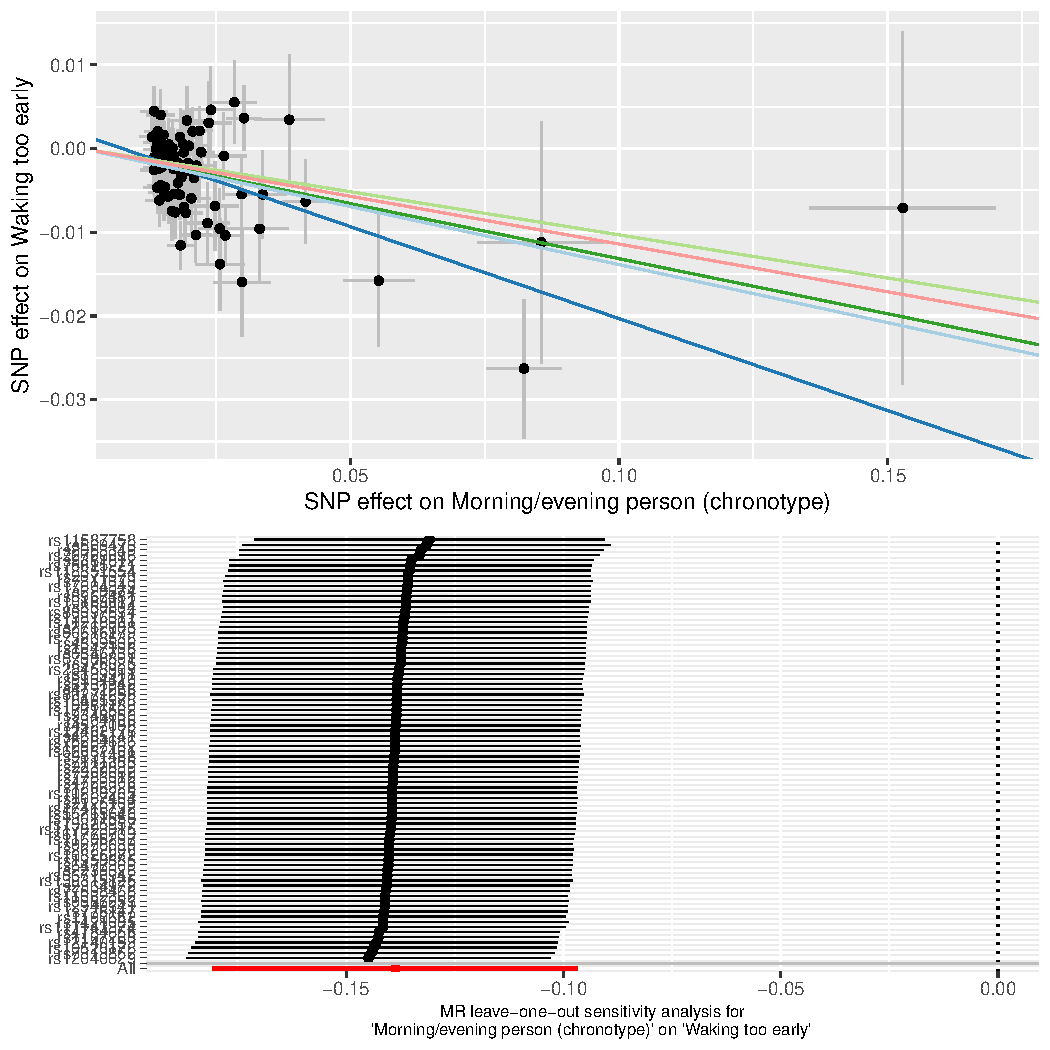
\includegraphics[width=\textwidth]{Figs/Analysis2/Morning_evening_person_(chronotype)_vs_Waking_too_early.Plots.pdf}
         \caption{}
         \label{waking}
     \end{subfigure}
        \caption{An evening chronotype contributes to increased serum testosterone (A) and a decrease in odds of waking early. IVW, Weighted median, mode, weighted mode, and Egger regressions shown. Lower panels depict leave-one-out sensitivity analyses with the IVW method.}
        \label{t2dmalcohol}
\end{figure}







\end{document}